%\subsection{Quo vadis studens?}
\subsection{Studienplanung im Bachelor}

Wie geht das eigentlich, studieren?\\
Wie du lernst, studierst, lebst; ob du brav mitschreibst oder öfter mal ausschläfst kannst und musst du selbst entscheiden. \\
Wann du die vorgeschriebenen Lehrveranstaltungen belegst, liegt ebenfalls in deinem eigenen Ermessen, allerdings: Nachdem bis auf vier Ausnahmen klar festgelegt ist was du studieren musst, ergibt sich eine sinnvolle Reihenfolge, da beispielsweise fortgeschrittenes Programmieren ohne Kenntnis von Algorithmen schlicht nicht möglich ist. Nichtsdestotrotz hast du Spielraum, das Studium an deine persönliche Situation anzupassen.
Du wohnst noch zu Hause und brauchst nicht arbeiten? Prima, mach noch Theoretische Informatik I im 1. Semester. Du hast ein Kind und musst nebenbei auch noch arbeiten? Kein Problem, sprich dich mit deinem Mentor ab und mach ein Teilzeitstudium. Die konkreten Vorschriften zum Studium findest du in der Prüfungsordnung.

In kurz: Grundsätzlich musst du Veranstaltungen im Wert von 180 Credit Points (CP) erfolgreich absolvieren, davon 116–121 CP im Bereich Informatik, 35 CP in Mathematik, 14–19 CP für dein Nebenfach und 10 CP für Schlüsselqualifikationen.

Um dir einen sinnvollen Weg durchs Studium zu ermöglichen, gibt es von der Fakultät den Musterstudienplan, der versucht Überschneidungen der Veranstaltungen zu vermeiden. Es gibt aber auch noch zwei Alternativstudienpläne der Fachgruppe, diese empfehlen wir dir allerdings nur, wenn du dir den geringen Mehraufwand pro Semester zutraust.

Auf den folgenden drei Seiten findet ihr die erwähnten Pläne. Der erste ist der Musterstudienplan der Fakultät. Der zweite Musterstudienplan gibt eine Orientierung, falls man das Fach Technische Informatik vorverlegen möchte. Der dritte Plan zeigt die Möglichkeit das Fach Theoretische Informatik vorzuverlegen. Bei beiden Plänen wurden zusätzliche Vorlesungen umgelegt, damit der Lernaufwand möglichst ausgeglichen bleibt. Theoretische Informatik und Technische Informatik bauen auf die Kenntnisse aus den Vorlesungen der ersten beiden Semester auf. Die Umlegung dieser Kurse nach vorne ist somit für diejenigen eine Möglichkeit, die schon vorher Kenntnisse gesammelt haben. Weitere Informationen, oder Erfahrungen bekommt ihr auf dem Treffen zum Stundenplanbau nach dem Erstsemesterfrühstück, oder bei einem Besuch im Fachgruppenraum der FG Informatik.

% Dafür wirst du es sehr genießen, während des SEPs und der Bachelorarbeit nicht so viele Vorlesungen zu haben. 
Du bist nicht mehr in der Schule, du hast nun Freiheiten, nutz sie weise und studiere so, wie du es für richtig hälst.!\\\\

\begin{figure}[p] 
		%\begin{center} 
  			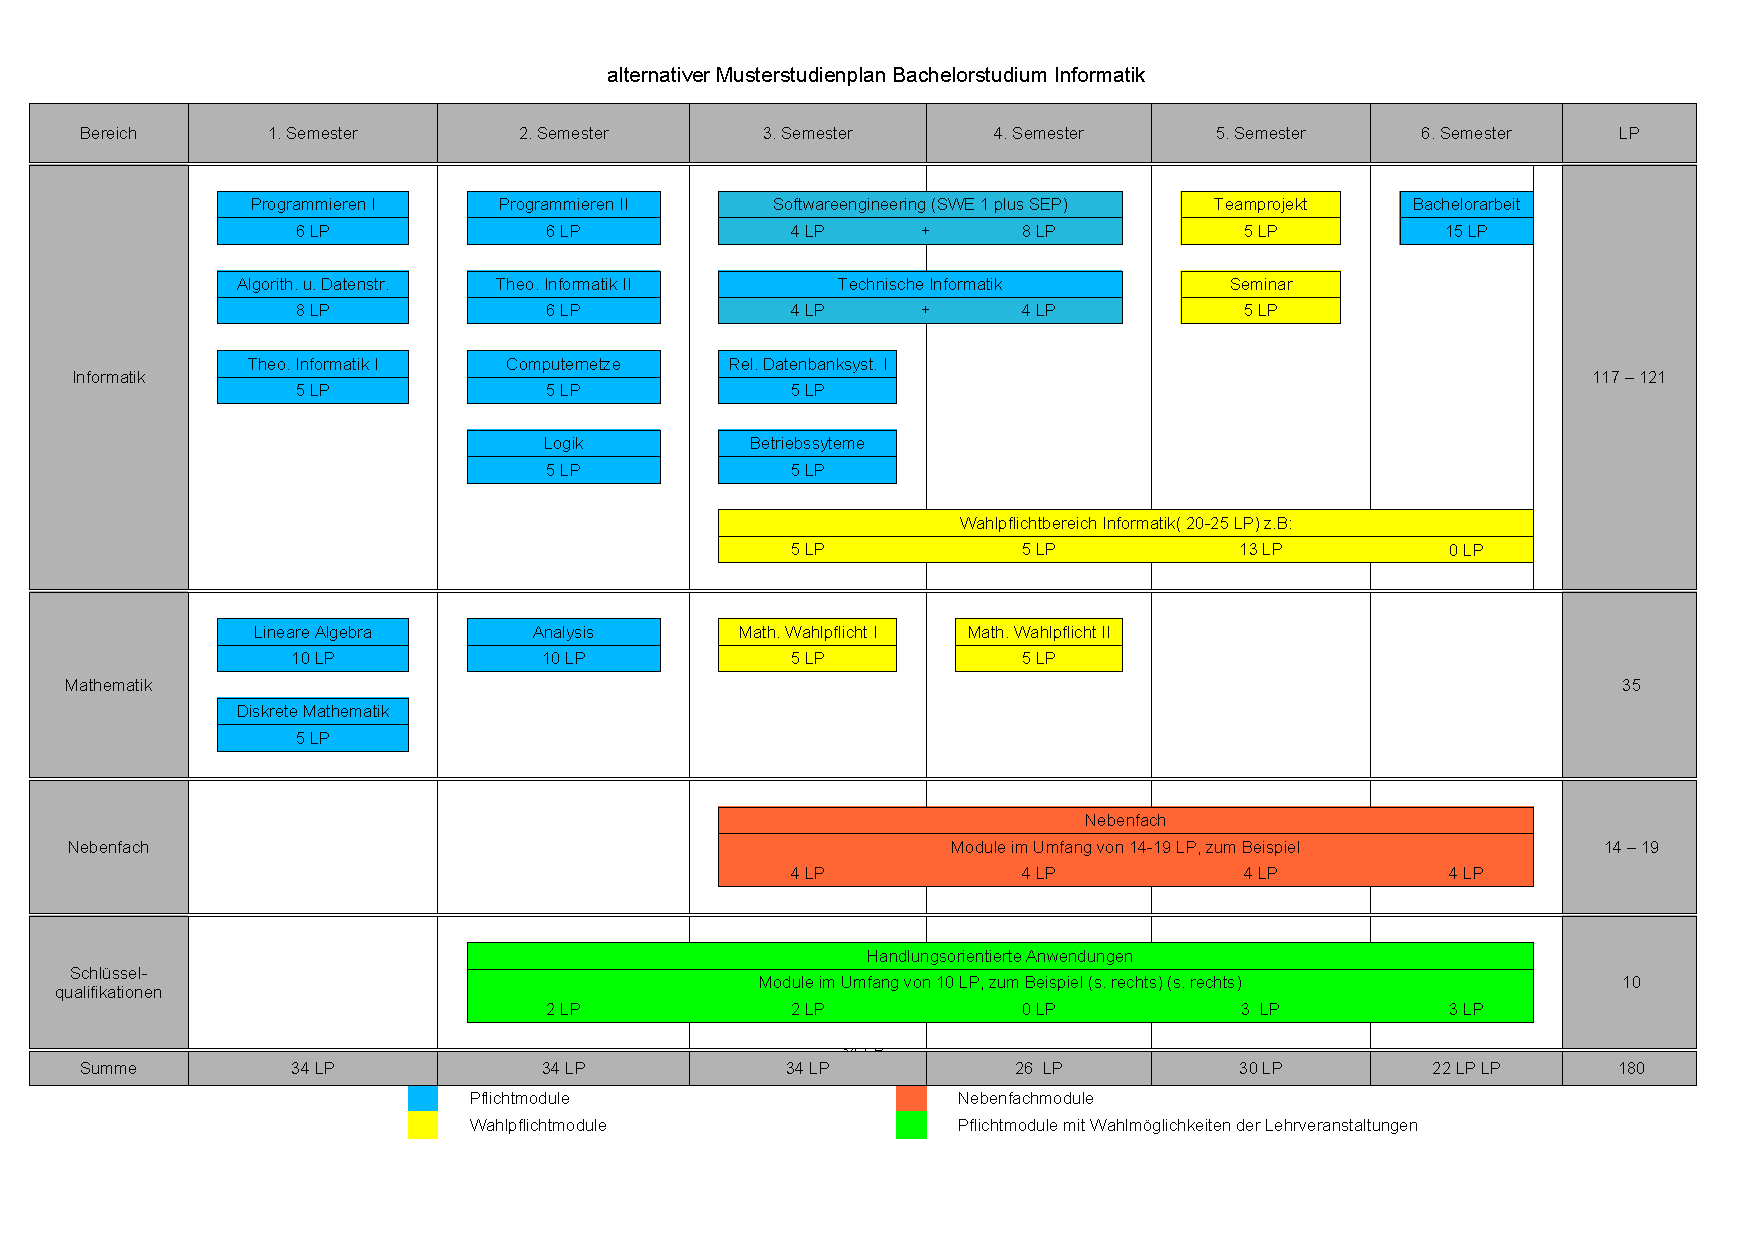
\includegraphics[angle=90, totalheight=\textheight, width=\textwidth ]
{bilder/studienplan_bsc_ws/studienplan_bsc}
				%{bilder/bachelortorte}
  			%\label{bachelortorte}
		\caption{Pflicht- und Wahlpflichtbereiche im Bachelor}
		%\end{center}
\end{figure}
